% -*- TeX:de -*-
\NeedsTeXFormat{LaTeX2e}
\documentclass[12pt,a4paper]{article}
\usepackage[german]{babel} % german text
\usepackage[DIV12]{typearea} % size of printable area
\usepackage[T1]{fontenc} % font encoding
%\usepackage[latin1]{inputenc} % most likely on Windows
\usepackage[utf8]{inputenc} % probably on Linux
\usepackage{multicol}

% PLOTTING
\usepackage{pgfplots} 
\usepackage{pgfplotstable}
\usepackage{url}
\usepackage{graphicx} % to include images
\usepackage{tikz}
\usepackage{subfigure} % for creating subfigures
\usepackage{amsmath} % a bunch of symbols
\usepackage{amssymb} % even more symbols
\usepackage{booktabs} % pretty tables

% a floating environment for circuits
\usepackage{float}
\usepackage{caption}

%\newfloat{circuit}{tbph}{circuits}
%\floatname{circuit}{Schaltplan}

% a floating environment for diagrams
%\newfloat{diagram}{tbph}{diagrams}
%\floatname{diagram}{Diagramm}

\selectlanguage{german} % use german

\begin{document}








%%%% TO DO
%
% - - Shorty:
%
% - Viskosität Stokes rechnen
% - Viskosität Höppler rechnen
% - Stokes und Höppler vergleichen
% 
% - Grafik vom Höpplerversuch

% - - Patrick
%
% - Einleitung viskosität
% - Skizze Stokes
% - Psychrometer
% - Skizze zum eiswasser




%%%%%%% DECKBLATT %%%%%%%
\thispagestyle{empty}
			\begin{center}
			\Large{Fakultät für Physik}\\
			\end{center}
\begin{verbatim}


\end{verbatim}
							%Eintrag des Wintersemesters
			\begin{center}
			\textbf{\LARGE WS 2013/14}
			\end{center}
\begin{verbatim}


\end{verbatim}
			\begin{center}
			\textbf{\LARGE{Physikalisches Praktikum\\ für das Bachelorstudium}}
			\end{center}
\begin{verbatim}




\end{verbatim}

			\begin{center}
			\textbf{\LARGE{PROTOKOLL}}
			\end{center}
			
\begin{verbatim}





\end{verbatim}

			\begin{flushleft}
			\textbf{\Large{Experiment (Nr., Titel):}}\\
							%Experiment Nr. und Titel statt den Punkten eintragen
			\LARGE{PW4 Oberflächenspannung, Viskosität, Hygrometrie, Schmelzwärme}	
			\end{flushleft}

\begin{verbatim}

\end{verbatim}	
							%Eintragen des Abgabedatums, oder des Erstelldatums des Protokolls
			\begin{flushleft}
			\textbf{\Large{Datum:}} \Large{31.10.2013}
			\end{flushleft}
			
\begin{verbatim}
\end{verbatim}
							%Namen der Protokollschreiber
		\begin{flushleft}
			\textbf{\Large{Namen:}} \Large{Patrick Braun, Johannes Kurz}
			\end{flushleft}

\begin{verbatim}


\end{verbatim}
							%Kurstag und Gruppennummer, zb. Fr/5
			\begin{flushleft}
			\textbf{\Large{Kurstag/Gruppe:}} \Large{DO/2}
			\end{flushleft}

\begin{verbatim}



\end{verbatim}
							%Name des Betreuers, das Praktikum betreute.
			\begin{flushleft}
			\LARGE{\textbf{Betreuer:}}	\Large{ Franz Sachslehner }	
			\end{flushleft}

%%%%%%% DECKBLATT ENDE %%%%%%%
\pagebreak
\setlength{\columnsep}{20pt}
\begin{multicols}{2}
\section{Einleitung}

\section{Oberflächenspannung}
Ziel des Experiments ist es, die Oberflächenspannung einer Flüssigkeit zu bestimmen. \\
Dazu wird ein Metallring an einer Waage befestigt, deren Skala mittels Gewichten geeicht wird. Taucht man den Ring in die Flüssigkeit und zieht den Flüssigkeitsbehälter langsam nach unten, kann beim Reißen der sich bildenden Flüssigkeitsmembran die dazu nötige Kraft an der Skala abgelesen werden.\\
Der Aufbau und die Eichgewichte sind in Abbildung \ref{fig:oberflaeche_eichung_aufbau} ersichtlich.\\


%\begin{figure}[H]
%	\centering
%	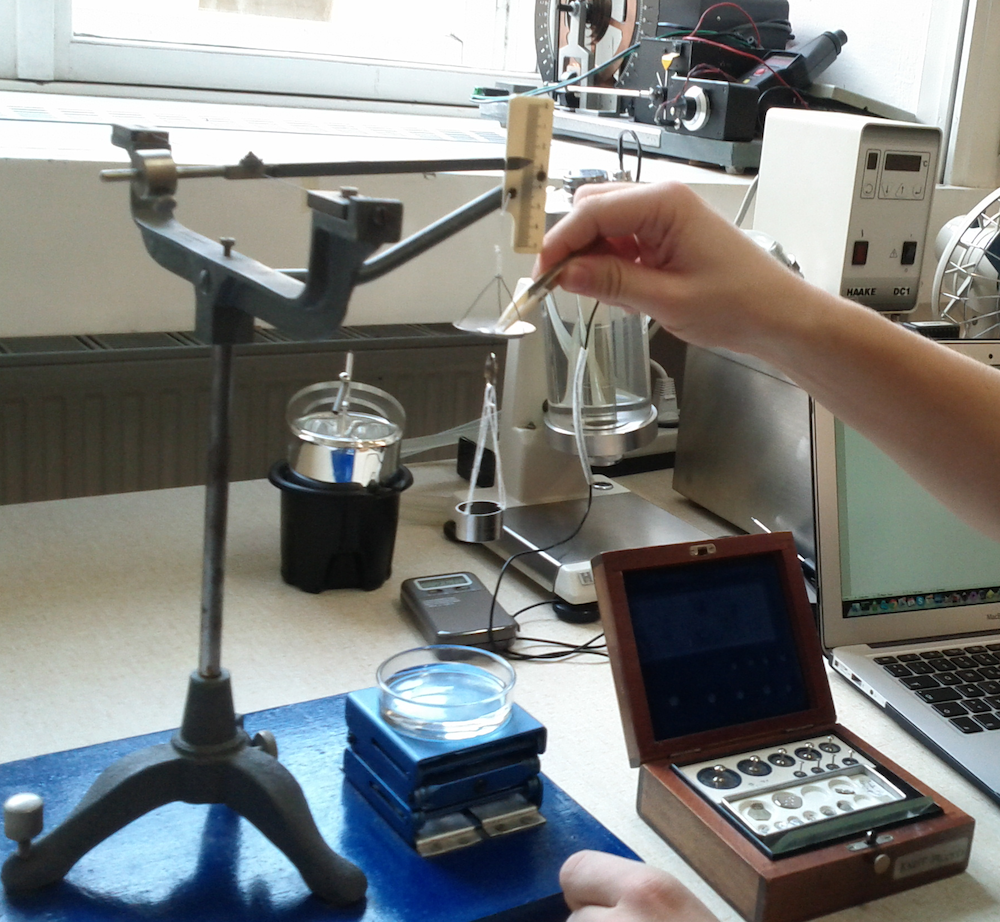
\includegraphics[scale=0.2]{./figure/Waageneichung-Aufbau.png}
%	\caption{Foto \\Versuchsaufbau und Eichung}
%	\label{fig:oberflaeche_eichung_aufbau}
%\end{figure}


\noindent
Bevor Messungen durchgeführt werden können, muss die verwendete Waage, wie beschrieben, geeicht werden. Dazu werden auf die Waagschale 0.1g schwere Metallstücke gelegt und die angezeigten Striche der Skala abgelesen. Dies wird von 0.1g bis 1.4g durchgeführt. Dadurch kann die Kraft pro Strich mit
$$K = m * a$$
errechnet werden. K ist ein empirischer Wert, den wir bei der Messung an der Skala ablesen.\\
Weiters ist die Oberflächenspannung abhängig vom mittleren Umfang des Ringes. Das Verhältnis zwischen Zugkraft und Umfang ergibt die Oberflächenspannung:
$$\sigma = \frac{K}{\pi * (d_1 + d_2)}$$

\noindent
Folgende Materialien wurden verwendet:
\begin{itemize}
	\item Eichgewichte
	\item Eine Pinzette
	\item Eine Waage
	\item Schale mit Wasser
	\item Metallring mit Aufhängung
	\item Ein beweglicher Objekttisch
	\item Ein Thermometer Sumit DT150
\end{itemize}

\noindent Bei der Durchführung wurde zuerst Leitungswasser, und danach destilliertes Wasser verwendet, um einen Vergleich zu ermöglichen.

\subsection{Messwerte und Ergebnisse}
Die Eichung der Waage ergab einen linearen Anstieg (Abbildung \ref{fig:oberflaeche_eichung_fit}). 

\begin{figure}[H]
	\centering
	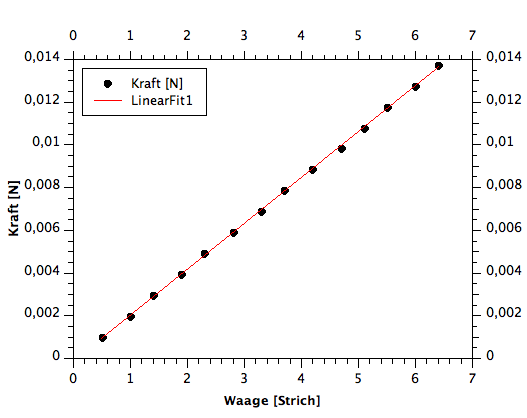
\includegraphics[scale=0.45]{./figure/Waageneichung-Fit_02.png}
	\caption{Skizze Versuchsaufbau}
	\label{fig:oberflaeche_eichung_fit}
\end{figure}


%%% TO DO ... komischer "02.png" Ausdruck in der Darstellung des pics... preview fehler?


\noindent
Durch den linearen Fit (Abbildung \ref{fig:oberflaeche_eichung_linreg}) der Messwerte (Tabelle \ref{fig:oberflaeche_eichung}) erhält man aus der Steigung die Kraft pro Skalenstrich. 
$$K = \frac{1}{465} = (2.200\pm 0.012)mN$$ 
Für den Metallring wurde mit einer Schiebelehre gemessen:\\
Außendurchmesser: $(24.00 \pm 0.05)mm$\\
Innendurchmesser: $(23.15 \pm 0.05)mm$\\
Oberflächenspannung $\sigma$ aus den Werten in Tabelle \ref{fig:oberflaeche_messung}:
$$\sigma = \frac{[Skalenstrich] * 0.0022N}{\pi * (0.02400 + 0.02315)m} $$ 
$$\sigma_{dest}= (68.62 \pm 0.36) \frac{mN}{m}$$ %TODO Fehler
$$ \sigma_{Leitg} = (57.92 \pm 0.33) \frac{mN}{m}$$



% Regress in Strich gegen N
%%%B (y-intercept) = -1,343535761669278e-04 +/- 4,628591085282343e-05
%%%A (slope) = 2,149302255457725e-03 +/- 1,174365191704868e-05


\begin{figure}[H]
	\centering
	\pgfplotstabletypeset[
			columns={g,strich},
			col sep=tab,
			columns/T1/.style={column name=$T_1[s]$},
			columns/T2/.style={column name=$T_2[s]$},
			every head row/.style={before row=\hline,after row=\hline\hline},
			every last row/.style={after row=\hline},
			every first column/.style={
								column type/.add={|}{}
							        },
			every last column/.style={
								column type/.add={}{|}
								}
			]{./data/oberflaechenspannung_eichung.dat}
	\caption{Eichungsmessung der Waage}
	\label{fig:oberflaeche_eichung}
\end{figure}
\noindent

\begin{figure}[H]
	\centering
	\pgfplotstabletypeset[
			col sep=space,
			every head row/.style={before row=\hline,after row=\hline\hline},
			every last row/.style={after row=\hline},
			every first column/.style={
								column type/.add={|}{}
							        },
			every last column/.style={
								column type/.add={}{|}
								}
			]{
			Wasser $Wasser_{destilliert}$
			3.9 4.7
			3.8 4.6
			3.9 4.6
			3.9 4.6
			3.9 4.6
			3.9 0
			4.0 0
			}
	\caption{Messung für destilliertes und Leitungs-Wasser in [Skalenstriche]}
	\label{fig:oberflaeche_messung}
\end{figure}

\noindent
Temperatur während der ersten Messung:\\
$T=(23.5 \pm 0.1)^{\circ}C$\\
Temperatur zweite Messung:\\
$T=(22.3 \pm 0.1)^{\circ}C$\\

\subsection{Diskussion}
Die Durchführung der Eichung und Messung gestaltete sich unproblematisch. Die Eichung erfordert etwas Fingerspitzengefühl und Geduld, da die Waage einen (fast) umgedämpften Oszillator gleicht.\\
Es ist zu berücksichtigen, dass die gemessene Kraft im Experiment, doppelt fehlerbehaftet ist:\\
Einerseits durch die Messung selbst in der Größenordnung der Skalenauflösung, andererseits durch den Umrechnungsfaktor der Waagenskala in Kraft. Diese Unsicherheit ist durch die lineare Regression der Eichwerte gegeben.\\


%%%%%%

In ersten Zwischenrechnungen ergab sich ein niedrigeres Ergebnis, als durch den Literaturwert erwartet:\\
$\sigma_{Wasser} = 72.75 \frac{mN}{m}$ bei $20^{\circ}C$\\
\\
Es wurde eine zweite Messreihe durchgeführt, mit destilliertem Wasser, um die Verunreinigungen so gering wie möglich zu halten (dabei ist auf eine sorgfältige Reinigung der Schale zu achten). \\
Außerdem war das destillierte Wasser ca. $1^{\circ}C$ kühler, also auch die Nebenbedingung Temperatur näher am verwendeten Literaturwert. Mit einem Ergebnis von $(68.62 \pm 0.36) \frac{mN}{m}$,  liegt diese Messung, bei $22.3^{\circ}C$, also auf einem, in guter Näherung, zu erwartenden Wert. Die Differenz ist hauptsächlich durch den Temperaturunterschied, und die Messungenauigkeiten der verwendeten Geräte, zu erklären. 

%%%%%%%%%%%%%%%%%%%%%%%%%%%%%%%%%%%%
\section{Viskosität}
In diesem Experiment ist es das Ziel, die Viskosität einer Flüssigkeit zu bestimmen. In einem einfachen Versuchsaufbau, wie aus Skizze \ref{fig:visko_aufbau} ersichtlich, wird eine Röhre mit der zu vermessenden Flüssigkeit gefüllt und Markierungen an der Außenseite angebracht. Danach wird die Distanz zwischen den Markierungen gemessen. \\
Probemassen in Kugelform dienen dazu, die Fallgeschwindigkeit in dem Fluid zu bestimmen. In der Röhre entsteht ein Gleichgewicht zwischen Auftrieb, Erdanziehung und Reibung. Berücksichtigt man dieses Gleichgewicht ergibt sich die folgende Gleichung:

$$\eta = \frac{(m-\rho \cdot V) \cdot g}{6 \cdot \pi \cdot v \cdot r \cdot \kappa}$$
m...Masse der Probe\\
$\rho$...Dichte der Flüssigkeit\\
V...Volumen der Kugel\\
g...Erdbeschleunigung (Lit.: $9.81m/s^2$)\\
v...Fallgeschwindigkeit (errechnet mit v = s/t)\\
r...Kugelradius\\
$\kappa$...Korrekturfaktor (siehe unten)\\
$$\kappa =  (1+2.1 * \frac{r}{R})$$
R...Röhrenradius\\
Flüssigkeit: 86\% iges Glyzerin\\
\\
Wichtig ist, bei diesem Versuch, alle Parameter zu bestimmen und dort, wo es möglich ist, Literaturwerte zu verwenden. \\
Der Korrekturfaktor ist nötig, da in der Gleichung von einer unendlichen Entfernung der Probe zum Rand des Flüssigkeitsvolumen ausgegangen wird. \\
Daher berücksichtigt der Korrekturfaktor das Verhältnis zwischen Kugelradius und Röhrenradius. Zuletzt bleibt nur noch, die Fallzeit der Probe zwischen den Markierungen zu messen, um die Geschwindigkeit v berechnen zu können.\\
Zur Durchführung der Messung wird mit der Pinzette eine Kugel genommen und in die Röhre geworfen. Es wird die Fallzeit zwischen den zwei Markierungen mit der Stoppuhr gemessen.
%%% TO DO Handskizze Stokesversuch
\begin{figure}[H]
	\centering
	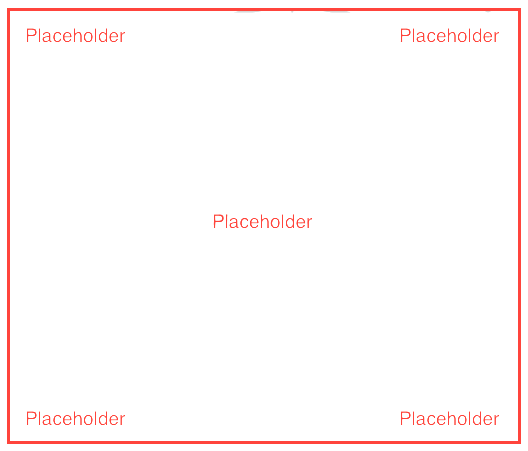
\includegraphics[scale=0.4]{./figure/placeholder.png}
	\caption{Skizze Kugelfallmethode nach Stokes}
	\label{fig:visko_aufbau}
\end{figure}

\textbf{Equipment:}\\
\begin{itemize}
	\item Eine Röhre mit Flüssigkeit
	\item Eine Pinzette
	\item Zwei verschiedene Kugelarten
	\item Eine Stoppuhr
	\item Ein Thermometer Sumit DT150
	\item HAAKE - Höppler-Viskosimeter mit Heizgerät
\end{itemize}
Außerdem soll die Viskosität des Glyzerins zum Vergleich mit dem Höppler-Viskosimeter gemessen werden, mit dem schließlich auch eine Messung bei höherer Temperatur durchgeführt werden soll.



\subsection{Messwerte und Ergebnisse}
Raumtemperatur: $(24 \pm 1)^{\circ}C$\\
\\
Fallstrecke: \\
\indent l = $(13.4 \pm 0.1)$ cm\\
%%%%%%%%%%%%%%% WERTE AUS TABELLE verwendet!!11einseinself
\noindent Dichte der Flüssigkeit: \\
\indent $\rho_{Glyz} = (1225 \pm 5) kg/m^2$\\
Radius des Zylinders:\\
\indent$R=15$ mm\\
\\
%Messung 2:\\
%$0.794 \pm 0.002mm$\\
%$16.1 \pm 0.1 mg$\\
%Messung 1:\\
%$6.6 \pm 0.1mg$\\
%$0.595 \pm 0.01mm$\\
Fallzeiten in $[s]$:
\begin{figure}[H]
	\centering
	\pgfplotstabletypeset[
			col sep=space,
			every head row/.style={before row=\hline,after row=\hline\hline},
			every last row/.style={after row=\hline},
			every first column/.style={
								column type/.add={|}{}
							        },
			every last column/.style={
								column type/.add={}{|}
								}
			]{
			Messung1 Messung2
			2.40 3.94
			2.37 3.97
			2.40 3.97
			2.38 4.13
			2.41 3.97
			2.41 3.97
			2.31 3.97
			2.44 3.79
			2.47 3.97
			2.44 3.88
			2.47 4.04
	}
	\caption{Messung der Fallzeiten}
	\label{fig:visko_fallzeit}
\end{figure}
\noindent

\noindent



\textbf{Messung 1:}\\
%Messung 1 Mean: 2,40909 \sigma 0,04657 Median: 2,41
$r_1 = (0.794 \pm 0.02) mm$\\
$m_1 = (16.1 \pm 0.1) mg$\\
$v_1 = (55.68 \pm 0.53)mm/s$\\
$\kappa_1 =  %(1+2.1 * \frac{0.794mm}{15mm}) = 
(1.1112\pm 0.0028)$\\
$$\eta_1 = %80.03\frac{mg}{mm*s} = 
(143 \pm 24) mPa \cdot s$$
\\
\noindent



\textbf{Messung 2:}\\
%Messung 2 Mean: 	3,98 \sigma 0,06197 Median: 4,13
$r_2=(0.595 \pm 0.01)mm$\\
$m_2=(6.6 \pm 0.1)mg$\\
$v_2 = (33.72 \pm 0.34) mm/s$\\
$\kappa_2 = %(1+2.1 * \frac{0.595mm}{15mm}) = 
(1.0833 \pm 0.0014)$\\

$$\eta_2 = %(0.2367 \pm xy)\frac{kg}{m s} = 
(131\pm 23) mPa\cdot s$$\\




\noindent
\textbf{Höppler-Viskosimeter}\\
%HAAKE, Thermometer, Heizgerät\\
(Raum-)Temperatur: $(25.0 \pm 0.1)^{\circ}C$\\
Messung 1: 171.19s\\
Messung 2: 171.32s\\
Messung 3: 171.32s\\
$t_{Raumtemp}= (171.28 \pm 0.05)s$\\
$$\eta_{Raumtemp}= (108.918\pm 0.90)mPa\cdot s$$
\\
(Heiz-)Temperatur: $(50.6\pm 0.1)^{\circ}C$\\
Messung 1: 42.25s\\
Messung 2: 41.63s\\
Messung 3: 41.78s\\
$t_{Heiztemp}= (41.89 \pm 0.19)s$\\
$$\eta_{Heiztemp}=(26.64\pm 0.17)mPa\cdot s$$

\subsection{Diskussion}
In die Messung der Viskosität einer Flüssigkeit gehen, je nach verwendeter Methode, viele Faktoren ein. Dabei haben vor allem die Abweichungen in Zusammensetzung und Temperatur der untersuchten Flüssigkeit große Auswirkungen auf das Ergebnis.\\
Das wird auch aus den durchaus unterschiedlichen Ergebnissen ersichtlich:\\
Vor allem der Vergleich zwischen $\eta_{Hoeppler}$ bei Raumtemperatur und den beiden Stokes-Kugelfallversuchen bietet wertvolle Ansätze: Die beiden Stokesmessungen haben, im Vergleich, relativ hohe Unsicherheitsbereiche, liegen jedoch innerhalb dieser gut beieinander. Die ermittelte Viskosität aus dem Höppler-Versuch liegt mit $(108.918\pm 0.86)mPa\cdot s$ gerade noch im Unsicherheitsbereich der 2. Stokesmessung und schon außerhalb der ersten.\\
Dabei sind, Ungenauigkeiten der Methodik beiseite gestellt, 2 Hauptquellen dieses Unterschiedes erkennbar:\\
- Es wurde nicht die gleiche Flüssigkeit verwendet\\
- die Temperatur war (um etwa $1^\circ$C) höher im Höppler-Versuch.\\
\\
Aus praktischen Gründen ließ sich das untersuchte 86\% ige Glycerin weder aus der einen Apparatur in die andere umfüllen, noch in irgendeiner Weise im Rahmen des Praktikums analysieren. Nimmt man dem Literaturwert für 100\% iges Glyzerin $(1480 mP \cdot s)$ zum Vergleich, lässt sich erkennen, dass dieser um eine ganze Größenordnung höher ist. Die Vermutung liegt also nahe, dass die Zusammensetzung der Flüssigkeit eine sehr große Rolle spielt.\\
Eine praktikable Möglichkeit, dem auf den Grund zu gehen wäre, die Daten aus allen Praktikumsgruppen zu vergleichen (insofern sie alle mit dem gleichen Glyzerin in Zylinder und Höppler-Viskosimeter arbeiten).\\
Die 2. Höpplermessung, bei ungefähr der doppelten Temperatur, liefert ein Ergebnis, eine Größenordnung niedriger, als bei Raumtemperatur. Auch hier zeigt sich also ein deutlicher Einfluss.\\
Hier hätte, mit dem Wissen aus der Auswertung, bereits beim Versuch auf bessere Temperaturkontrolle geachtet werden sollen, um die Messung zu optimieren.\\
\\
Vor allem aber auch im Stokes-Versuch ergeben sich noch eine Reihe andere Fehlerquellen:\\
Die Fallzeit wird von Hand gemessen, sowie der Beginn des Fallweges mit den Augen abgeschätzt. Das wäre sicherlich durch weitere Übung noch zu optimieren. Tatsächlich geht die Unsicherheit aus der Geschwindigkeit eher durchschnittlich in die Fehlerfortpflanzung ein.\\
Besonders groß (2 Größenordnungen höher als der Durchschnitt) ist der Effekt der Unsicherheiten der Flüssigkeitsdichte $\rho$ sowie der Kugelradien $r_1$ und $r_2$ (Beide wurden aus der Angabe übernommen).\\
Daher lässt sich vermuten, dass die Methodik des Stokes-Versuches (im Rahmen einer größeren Unsicherheit) durchaus gute Ergebnisse liefert und vor allem die Unterschiede in den Versuchsbedingungen (Flüssigkeit und Temperatur) zu den, nicht ganz, deckungsgleichen Ergebnissen geführt haben.\\
Die erwähnten Optimierungen, gemeinsam mit der Auswertung mehrerer Testreihen, würden zu weiteren Erkenntnissen über die Abhängigkeiten in diesem Experiment führen.





%%%%%%%%%%%%%%%%%%%%%%%%%%%%%%%%%%%%
\section{Luftfeuchtigkeit}
\textbf{Equipment}
\begin{itemize}
	\item Psychrometer mit Gazestrumpf
	\item Ein Ventilator
	\item ULab Datalogger
	\item Relative Humidity sensor
\end{itemize}

\noindent In diesem Versuch soll die Luftfeuchtigkeit einerseits mittels eines Aspirationspsychrometers, und andererseits durch ein digitales Messgerät gemessen werden.\\
Das Psychrometer bestimmt die Luftfeuchtigkeit indem die Verdunstungskälte gemessen wird: 2 baugleiche Quecksilberthermometer befinden sich in unmittelbarer Nähe. Über das eine ist befeuchteter Stoff gewickelt. Das Wasser verdunstet bis die umgebende Luft mit Feuchtigkeit gesättigt ist und die Temperatur im Gleichgewicht ist. Es wird ein Luftstrom erzeugt, der die gesättigte Luft abführt um die Temperatur konstant zu halten. Aus der Differenz der Temperaturen am trockenen ($T_t$) und am feuchten Thermometer ($T_f$), kann die absolute Luftfeuchtigkeit, $\rho_w$, sowie die relative, $\phi$, berechnet werden:\\
$$\rho_w=\frac{p_w(T_t)\cdot M_w}{R \cdot T_t}$$
$$\phi= \frac{p_w(T_t)}{p_{w,max}(T_t)}100\%$$
wobei:
$$p_w(T_t)=p_{w,max}(T_t)-67 Pa/K \cdot (T_t-T_f)$$
und $p_{w,max}(T_t)$ einer Tabelle entnommen wird.\\
In den Faktor $67Pa/K$ gehen die molaren Massen von Luft und Wasser ein, der Luftdruck auf Meereshöhe, die Wärmekapazität von Luft sowie die Verdampfungswärme von Wasser.

\subsection{Messwerte und Ergebnisse}
\begin {itemize}
	\item Temperaturen\\
	$T_{t} = (24 \pm 1)^{\circ}C$\\
	$T_{f} = (17 \pm 1)^{\circ}C$\\
	T vor dem Versuch:\\
	$(24 \pm 1)^{\circ}C$\\
\end{itemize}

$$\rho_w= (132 \pm 14)g/m^3$$
$$\phi =(49.2\pm 3.2)\%$$
\\
Messung mit ULab:
$$\phi_{digi}=(47 \pm 1)\%$$

\subsection{Diskussion}

Die gemessenen Werte aus beiden Methoden stimmen miteinander überein, sogar insofern, dass der kleinere Unsicherheitsbereich aus der Digital-Messung komplett innerhalb des etwas größeren aus der Psychrometermessung liegt.\\
Die Temperaturen am Psychrometer bleiben während der Messung im sichtbaren Bereich stabil, es wäre also vorstellbar, mit genauerer Skalierung, auch mit dieser Methode noch etwas genauere Ergebnisse zu erzielen.\\


%%%%%% EIS - SCHMELZWAERME %%%%%%%%

\section{Schmelzwärme vonEis}
Bei der Wärmezufuhr in einen Stoff kommt es bei Phasenübergängen zu Zeiten konstanter Temperatur, währendderer die zugeführte Energie zur Gänze in die Zustandsänderung, nicht jedoch in die Temperaturänderung geht.\\
\\
In diesem Versuch soll die spezifische Schmelzwärme von Eis (Wasser aus der Haushaltsleitung, Wien) bestimmt werden. Es wird dazu die Mischungsmethode verwendet:\\
In einem (idealerweise völlig) wärmeisolierten Gefäß werden 2 Stoffe unterschiedlicher Temperatur gemischt. Die abgegebene Wärmemenge des wärmeren Stoffes muss wegen der Energieerhaltung gleich der aufgenommenen Wärmemenge des kälteren und des Gefäßes sein.\\
Aus den Anfangstemperaturen und der Mischtemperatur lässt sich beispielsweise auf die latente Wärme schließen, die beim Schmelzvorgang von Eis frei wird.
$$\Delta Q_1=(C_k+m_wc_w)(T_1-T_m)=$$
$$=\Delta Q_2 = m_eS+m_ec_w(T_m-T_S)$$
$S$ ist die gesuchte spezifische Schmelzwärme des Eises, die Massen $m_e$, $m_w$ des verwendeten Wasser und Eises sowie die Wärmekapazitäten $c_w$, $C_k$ von Wasser und dem verwendeten Gefäß gehen in die Rechnung ein.\\

%%%% TO DO Handskizze Kalorimeter

\noindent Equipment:
\begin {itemize}
	\item Ein Kalorimetergefäß mit Rührer
	\item Wasser und Eis
	\item Ein ULab-Datalogger mit Temperatursonde
\end {itemize}

Das Kalorimeter wird, zu etwas mehr als der Hälfte, mit erhitztem Wasser (ca. $80^{\circ}$ C) gefüllt und der Temperaturverlauf des Systems wird mehrere Minuten gemessen.\\
Nach ein paar Minuten wird Eis eingebracht (weniger als Wasser). Es ist darauf zu achten, das Eis schnell einzuwerfen und sofort und durchgehend zu rühren um den Schmelzvorgang zu beschleunigen.\\
Schließlich soll ein instantaner Temperaturausgleich approximiert werden.\\
Während des gesamten Versuchs wird der Temperaturverlauf gemessen, der grob in 3 Abschnitte geteilt werden kann, die durch Anlegen von Geraden idealisiert werden (vgl. Abb. \ref{fig:Tempverlauf-Eis}):\\
- Vor der Zugabe von Eis\\
- während des Schmelzvorganges\\
- nach der Vermischung


\end{multicols}

%%%% Diagramm Eis
\begin{figure}[H]
	\centering
	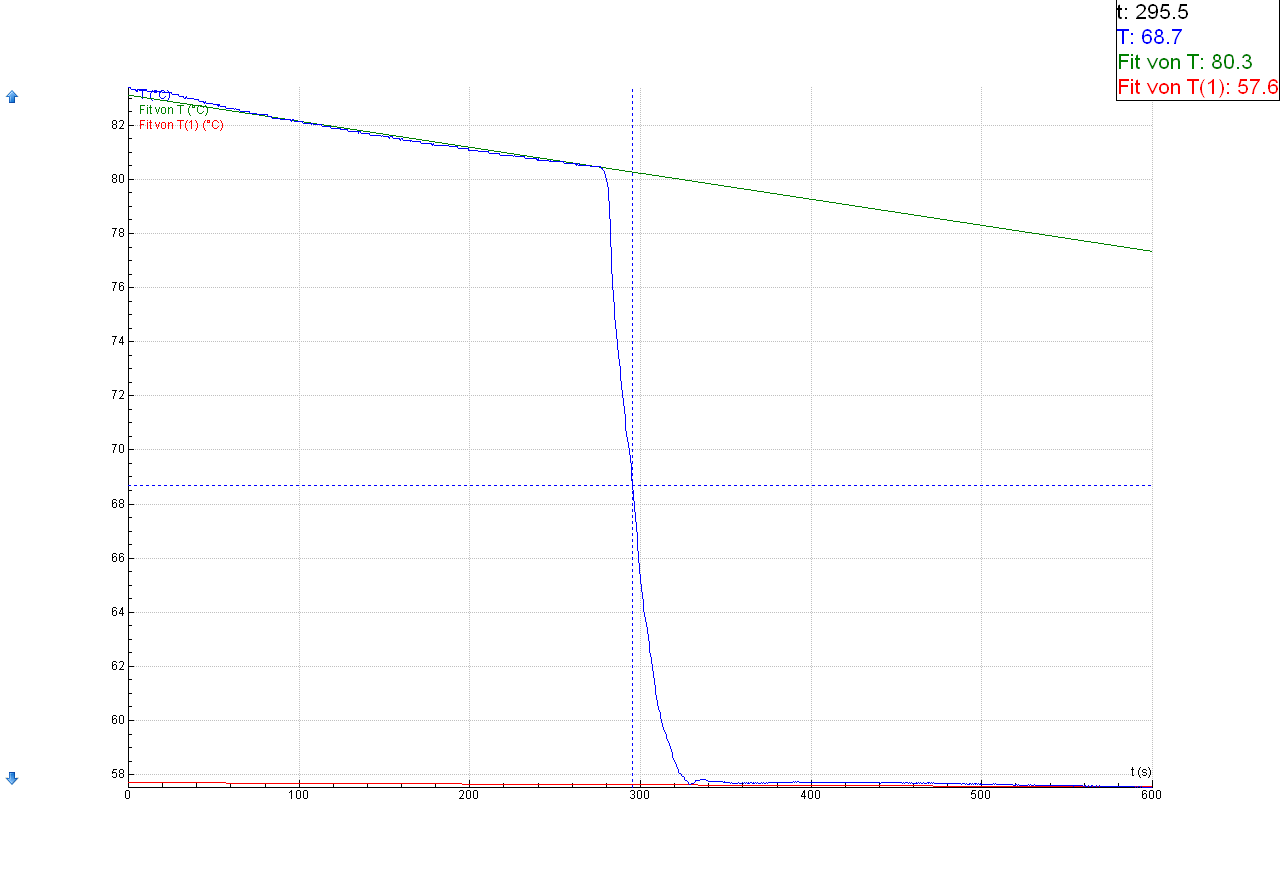
\includegraphics[scale=0.35]{./figure/PW4_graph.PNG}
	\caption{Temperatur in [$^\circ$C] gegen die Zeit in [s] im Kalorimeter\ }
	{\centering Screenshot aus Coach6}
	\label{fig:Tempverlauf-Eis}
\end{figure}
\noindent

\begin{multicols}{2}


\subsection{Messwerte und Ergebnisse}

\begin{itemize}
	\item Wärmekapazitäten:\\
	Kalorimeter: $C_k = (100 \pm 10) J/K$\\
	Wasser (20$^{\circ}$C): $c_w=(4,182) J/gK$
	
	\item Massen:\\
	Kalorimeter: $(236.6 \pm 0.1)g$\\
	Wasser: $m_w = (154.0 \pm 0.2)g$\\
	Eis: $m_e = (26.0 \pm 0.2)g$
	
	\item Temperaturen:\\
	Anfang: $T_1=(80 \pm 1) ^\circ C$\\
	Ende: $T_m=(58 \pm 1) ^\circ C$\\
	Schmelztemp. Eis: $T_S = 0 ^\circ C$
\end{itemize}

\noindent spezifische Schmelzwärme von Wasser:\\
$$S =(387 \pm 45) kJ/kg$$

\subsection{Diskussion}
Der Literaturwert der spezifischen Schmelzwärme von Eis von 333.5 KJ/kg liegt außerhalb des Unsicherheitsbereichs dieser Messung:\\
Die angewandte Methode bietet, trotz computergestützter Messung, einige mögliche Fehlerursachen:\\
Die horizontalen Geraden in Abb \ref{fig:Tempverlauf-Eis} wurden "von Hand" gefittet und die Flächen links und rechts der senkrechten Schnittgerade als gleich abgeschätzt. Hier sind sicherlich Verbesserungen möglich, auch wenn die Fehlerabschätzung von $\pm 1 ^\circ C$ bei beiden Temperaturen bewusst groß gewählt ist, um dem Problem gerecht zu werden.\\
\\
Eine andere Fehlerquelle hat sich sehr deutlich in einem ersten Versuch gezeigt, in dem sowohl das Einbringen der Eiswürfel sehr zögerlich und langsam durchgeführt wurde, als auch vergessen wurde, zu rühren, um die Vermischung zu beschleunigen. Dadurch ergaben sich unerwartete und große Temperaturschwankungen im Schmelzzeitraum und das Experiment musste wiederholt werden.\\
Es ist also durchaus möglich, dass das Öffnen der Abdeckung zum Eiswürfel-Input, und andere Manipulationen am System (rühren, messen, Wärmeleitung des Kalorimeters, u.a.) auch zu Verzerrungen der Messung führen.\\
Eine weiterer, in dieser Durchführung nicht kontrollierter Parameter in diesem Experiment ist das verwendete Wasser: Es wurde Wasser aus der Wiener Haushaltswasserleitung verwendet, ohne etwaige Bestandteile genauer zu ermitteln. Das Wasser wurde erhitzt im Wasserkocher der Praktikumsräume, auch hier sind Verunreinigungen nicht auszuschließen.\\
Um also den Einfluss einzelner der erwähnten Fehlerquellen zu bestimmen und diese zu minimieren, wären also weitere Versuche, unter verschiedenen Bedingungen, nötig. Beispielsweise könnte das Experiment mit destilliertem Wasser durchgeführt werden, die gemessenen Daten mit unterschiedlichen Programmen ausgewertet und die Durchführung durch Übung und Verwendung eines anderen Gefäßes beschleunigt werden.


\section{Quellen}
\noindent Oberflächenspannung von Wasser:\\
\url{http://de.wikipedia.org/wiki/Oberfl%C3%A4chenspannung}\\
\noindent spezifische Wärmekapazität von Wasser:\\
\url{http://de.wikipedia.org/wiki/Spezifische_W%C3%A4rmekapazit%C3%A4t}
\noindent Viskosität von Glyzerin und ihr temperaturabhängiger Verlauf:\\
\url{http://de.wikipedia.org/wiki/Viskosit%C3%A4t}

\end{multicols}
\end{document}